

\begin{enumerate}
\item Browse to the directory where you saved the setup file when you downloaded \app{}. 
\item Double-click the file \bxcaption{setup.exe}. 
\item A welcome screen appears (\bxfigref{figWelcome}). Click \bxcaption{Next} to begin installation. 

\begin{center}
\begin{figure}[h]
  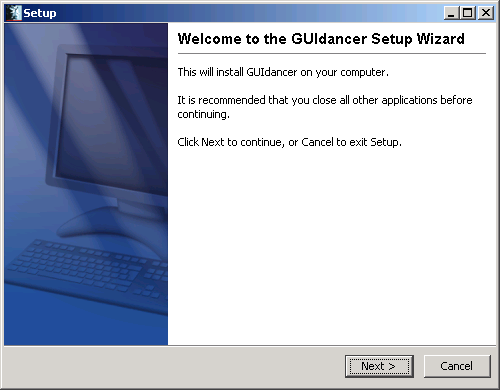
\includegraphics[width=10cm]{Windows/PS/welcome}
  \caption{Welcome Screen}
  \label{figWelcome}
\end{figure}
\end{center}


\item The license agreement will appear. Read it and accept it to continue.  
You can view and print this license later. It is saved in the \app{} installation directory and is called \bxname{license-agreement.txt}. 
\item At the next dialog, choose where to install \app{}. You can search or enter a directory or use the default. Click \bxcaption{Next}.
\item Choose the components to be installed (\bxfigref{figComponents}).
You can install the \gdagent and the client on different machines if you want to.  If this is the case, carry out the installation for the other component (\gdagent or client) later. 

To be able to access the manual as a .pdf file and to  print it  out, install the  \app{} documentation. Click \bxcaption{Next}.
 
\begin{center} 
\begin{figure}[h]
  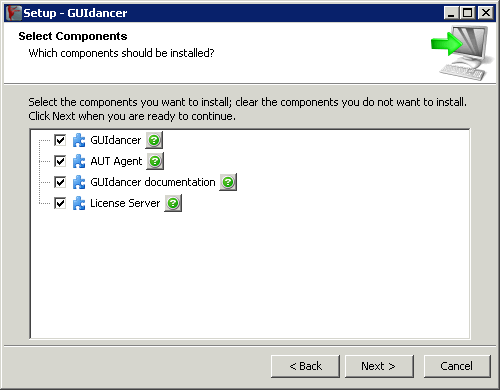
\includegraphics[width=10cm]{Windows/PS/components}
  \caption{Component Selection}
  \label{figComponents}
\end{figure}
\end{center}

\item Choose a start menu folder to create the shortcuts in. If you are installing as an administrator, there is a checkbox with the option to install the shortcuts for all users. To continue, click
\bxcaption{Next}. 
\item The selected components will  be installed.
\item Once the installation is finished, a dialog appears to confirm this (\bxfigref{complete}).

\begin{center}
\begin{figure}[h]
  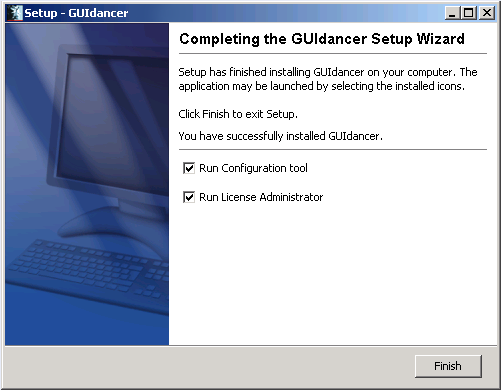
\includegraphics[width=10cm]{Windows/PS/complete}
  \caption{Installation complete}
  \label{complete}
\end{figure}
\end{center}

From this dialog you can also opt to start the configuration tool
% \gddb initialization
 and license administrator after finishing the installation
process. 

We recommend starting the license administrator automatically, especially if you are a first-time user. If you want to  customize your installation, it is a good
idea to run the configuration tool before using 
%the CreateDB tool or 
the license administrator. See later \bxpref{custInst} for details on the configuration tool. 

 
\bxtipp{Configuration details can also be changed at a later point. The configuration tool is in the  \app{} start menu folder: \\
\bxmenu{\gd}{Admin}{GDConfiguration}. }

\item Click \bxcaption{Next} and then \bxcaption{Finish} to exit the installation wizard. 
\item You can  now use the configuration tool (optional),
% and you must create a database using the createDB tool, 
and you must then start the license administrator to request and add licenses.  

\end{enumerate}




